\chapter{Criptografía y Curvas Elípticas:}
%\noindent\rule[-1ex]{\textwidth}{2pt}\\[4.5ex]

En este capítulo se introducirá la teoría sobre criptografía y curvas elípticas necesaria para entender la base detrás de los criptosistemas usados en las aplicaciones de mensajería más populares.

\section{Introducción a la criptografía}
En este apartado voy a hablar sobre los objetivos de un criptosistema y los posibles ataques que se le pueden hacer, así como una introducción a la criptografía simétrica y asimétrica y su uso en las aplicaciones de mensajería que nos ayudará a entender los distintos criptosistemas de los que se hablará después.
Mayormente la información de este apartado ha sido obtenida de \cite{GomezPardo2002b} para los criptosistemas simétricos y \cite{angelRiosMateos} para los cifrados asimétricos.\\

Los principales objetivos que debe cumplir todos los criptosistemas son:
\begin{itemize}
		\item \textbf{Confidencialidad} la información solo puede ser accesible por las entidades autorizadas. 
		\item \textbf{Integridad} la información no ha sido alterada en el envío.
		\item \textbf{Autenticidad} la información proviene de quién afirma haberla enviado.
		\item \textbf{No repudio} el emisario de una información no puede a posteriori negar que se realizado tal envío.
\end{itemize}

Para hablar de los ataques supondremos que se sigue el principio de \emph{Kerckhoffs}, el cual establece que el adversario conoce todos los detalles del criptosistema excepto la clave empleada.\\
Los posibles ataques son:
\begin{itemize}
		\item \textbf{Criptograma} el adversario conoce el criptograma, es decir, el mensaje cifrado o un fragmento de este.
		\item \textbf{Mensaje Conocido} el atacante conoce parejas mensaje/criptograma cifradas con una misma clave.
		\item \textbf{Mensaje escogido} el atacante puede generar criptogramas para mensajes de su elección. Una vez obtenidas dichas parejas, trata de averiguar el mensaje correspondiente a un criptograma desconocido.
		\item \textbf{Mensaje escogido-adaptativo} el atacante no solo puede generar pareas mensaje/criptograma a su elección, sino que puede hacerlo tantas veces como quiera realizando los análisis que considere oportunos.
		\item \textbf{Criptograma escogido y escogido-adaptativo} similar a los anteriores pero partiendo del criptograma, teniendo acceso a descifrar los criptogramas que desee, inicialmente o a lo largo del proceso. Lo que se busca en este ataque es la clave.
\end{itemize}

Una vez vistos los objetivos que tienen que cumplir los criptosistemas y los posibles ataques veamos qué son los criptosistemas simétricos y asimétricos y su uso en las aplicaciones de mensajería.\\

\subsection{Cifrado simétrico}
Criptosistema en el cual se utiliza una sola clave para cifrar y descifrar un mensaje. Lo más importante para la seguridad de los criptosistemas es la propia clave mientras que el algoritmo en si mismo, no es tan importante como medida de seguridad. Es decir, lo importante es que el atacante no conozca la clave, mietras que conozca el algoritmo usado no lo es tanto.\\
Un criptosistema simétrico está formado por:
\begin{itemize}
	\item $\mathcal{M}$ el conjunto de los mensajes.
	\item $\mathcal{C}$ el conjunto de los criptogramas.
	\item $\mathcal{K} \subseteq \mathcal{K}_p\times\mathcal{K}_s$ el espacio de las claves. 
\end{itemize}
Un criptosistema simétrico viene definido por dos aplicaciones
$$E:\mathcal{K}_p\times\mathcal{M}\rightarrow\mathcal{C}$$
$$\mathcal{D}:\mathcal{K}_s\times\mathcal{C}\rightarrow\mathcal{M}$$
tales que para cualquier clave $k_p \in \mathcal{K}_p$, existe una clave $k_s$ de manera que dato cualquier mensaje $m \in \mathcal{M}$,
$$
\mathcal{D}(k_s,E(k_p,m))=m.
$$
Fijada la clave $k_p \in \mathcal{K}_p$ y su correspondiente $k_s \in \mathcal{K}_s$ se definen las funciones de cifrado y descifrado como:\\
\begin{aligned}
	\center
	&$E_{k_p}:\mathcal{M}\rightarrow\mathcal{C}$\\
	&$E_{k_p}(m)=E(k_p,m)$
\end{aligned}
\begin{aligned}
	\center
	&$D_{k_p}:\mathcal{C}\rightarrow\mathcal{M}$\\
	&$D_{k_s}(c)=D(k_s,c)$
\end{aligned}

\subsection{Cifrado asimétrico}
Criptosistema en el cual se utilizan dos claves, una para cifrar el mensaje y otra para descifrarlo. La clave para cifrar es la que se conoce como \emph{clave pública} mientras que la que se utiliza para descifrar es la \emph{clave privada}. Estos criptosistemas surgieron para paliar la debilidad de los criptosistemas simétricos, que es que la clave que cifra y descifra se tiene que compartir, pudiendo esta ser interceptada.  La seguridad de estos criptosistemas reside en que no se conozcla la clave privada.\\
Un criptosistema asimétrico está formado por:
\begin{itemize}
	\item $\mathcal{M}$ es el conjunto de los mensajes.
	\item $\mathcal{C}$ es el conjunto de los criptogramas.
	\item Una función $P:\mathcal{K}' \rightarrow \mathcal{K}$, que nos permitirá generar la clave pública.
\end{itemize}
Un criptosistema asimétrico viene definido por dos aplicaciones:
$$E:\mathcal{K}\times\mathcal{M}\rightarrow\mathcal{C}$$
$$\mathcal{D}:\mathcal{K}'\times\mathcal{C}\rightarrow\mathcal{M}$$
tales que para cualquier clave privada $k' \in \mathcal{K}'$ obtenemos la clave pública como $P(k')=k$ y se definen las funciones de cifrado y descifrado como:\\
\begin{aligned}
	\center
	&$E_{k}:\mathcal{M}\rightarrow\mathcal{C}$\\
	&$E_{k}(m)=E(k,m)$
\end{aligned}
\begin{aligned}
	\center
	&$D_{k^{'}}:\mathcal{C}\rightarrow\mathcal{M}$\\
	&$D_{k'}(c)=D(k',c)$
\end{aligned}

Para que un criptosistema asimétrico sea seguro tenemos que garantizar:
\begin{itemize}
	\item $P$ es una función de dirección única, es decir, que dado un elemento de su imagen no se puede calcular su imagen inversa fácilmente.
	\item Para la mayoría de los $k \in \mathcal{K}$, la aplicación $E_k$ es de dirección única.
	\item $\mathcal{D}_{k'}$ se puede calcular en un periodo corto de tiempo si se conoce $k'$ y que sea imposible o el periodo sea muy largo en caso de solo conocerse $k$.
\end{itemize}

\subsection{Criptosistemas simétricos y asimétricos en las aplicaciones de mensajería}
Ambos tipos de criptosistemas son muy utilizados en las aplicaciones de mensajería de manera complementaria.\\ 
Los criptosistemas simétricos debido a su velocidad de cifrado, su uso reducido de recursos y su mejor manejo de grandes cantidades de datos se suelen utilizar para cifrar los mensajes. 
Pero como tienen el defecto de que si la clave es interceptada el criptosistema es vulnerado y se pierde tanto la confidencialidad como la autenticidad de los mensajes.\\ 
Para evitar esto se suele complementar con métodos seguros para el intercambio de la clave como puede ser el \emph{intercambio de claves Diffie-Hellman}.\\
Loss cifrados asimétricos son muy utilizados para la firma y autentificación de los mensajes, garantizando de esta manera la seguridad de la aplicación y una eficiencia mucho mayor que si se utilizara únicamente un criptosistema asimétrico.\\
A continuación se introducirá los cifrados de bloque, necesarios para enteder el algoritmo \textbf{Rindael AES} que se explicará posteriormente.

\subsection{Cifrados de bloque}
Son criptosistemas de clave simétrica en los que la longitud de los bloques y claves es fija.\\
Este criptosistema se define
$$
	E:\mathbb{B}^K\times\mathbb{B}^N\rightarrow \mathbb{B}^N,
$$
$$
	D:\mathbb{B}^K\times\mathbb{B}^N\rightarrow \mathbb{B}^N,
$$
Donde N es el tamaño del bloque y K es el tamaño de la clave.\\
Los cifrados tienen distintos modos de operación los cuales dependen solo del tamaño del bloque, estos son:\\
\begin{itemize}
	\item \textbf{Electronic CodeBook}
	\begin{itemize}
		\item \textbf{\emph{Cifrado ECB}}
		\begin{description}
			\item Dividimos m en $m_{[1]}...m_{[l]}$ con $m_{[i]} \in \mathbb{B}^N$
			\item Para i=1,...,l hacer
			\begin{description}
				\item $c_{[i]} = E_k(m_{[i]})$
			\end{description}
			\item Devolvemos $c_{[1]}...c_{[l]}$
		\end{description}

		\item \textbf{\emph{Descifrado ECB}}
		\begin{description}
			\item Dividimos c en $c_{[1]}...c_{[l]}$ con $c_{[i]} \in \mathbb{B}^N$
			\item Para i=1,...,l hacer
			\begin{description}
				\item $m_{[i]} = D_k(c_{[i]})$
			\end{description}
			\item Devolvemos $m_{[1]}...m_{[l]}$
		\end{description}
	\end{itemize}

		\begin{figure}[htb]
			\centering
			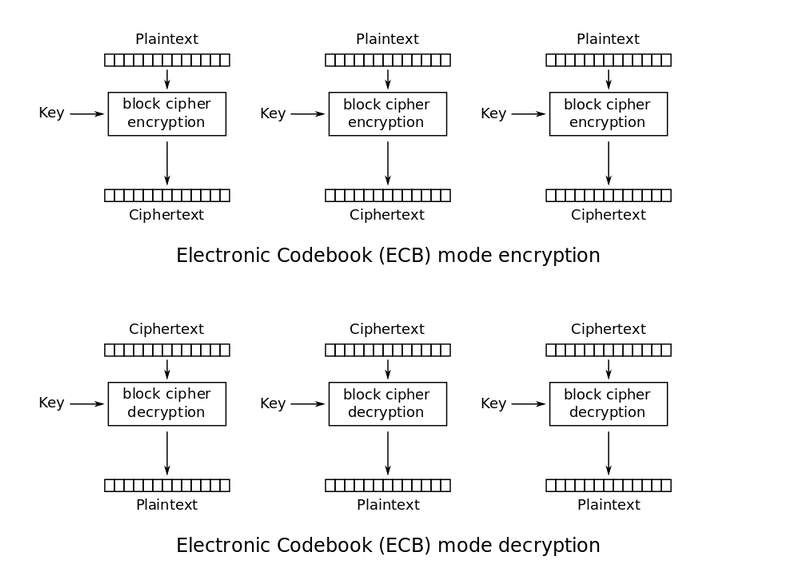
\includegraphics[scale=0.4]{imagenes/ecb.png} 
			\caption{Esquema del cifrado y descifrado del modo ECB \cite{cifradobloque}.}
			\label{esquemaecb}
		\end{figure}
		
	\item \textbf{Cipher-Block Chaining}
	\begin{itemize}
		\item \textbf{\emph{Cifrado CBC}}
		\begin{description}
			\item $c_{[0]} \in \mathbb{B}^*$
			\item Dividimos m en $m_{[1]}...m_{[l]}$ con $m_{[i]} \in \mathbb{B}^N$
			\item Para i=1,...,l hacer
			\begin{description}
				\item $c_{[i]} = E_k(m_{[i]}\oplus c_{[i-1]})$
			\end{description}
			\item Devolvemos $c_{[1]}...c_{[l]}$
		\end{description}

		\item \textbf{\emph{Descifrado CBC}}
		\begin{description}
			\item Dividimos c en $c_{[0]}...c_{[l]}$ con $c_{[i]} \in \mathbb{B}^N$
			\item Para i=1,...,l hacer
			\begin{description}
				\item $m_{[i]} = D_k(c_{[i]})\oplus c_{[i]}$
			\end{description}
			\item Devolvemos $m_{[1]}...m_{[{l}]}$
		\end{description}
	\end{itemize}
%\newpage
		\begin{figure}[htb]
			\centering
			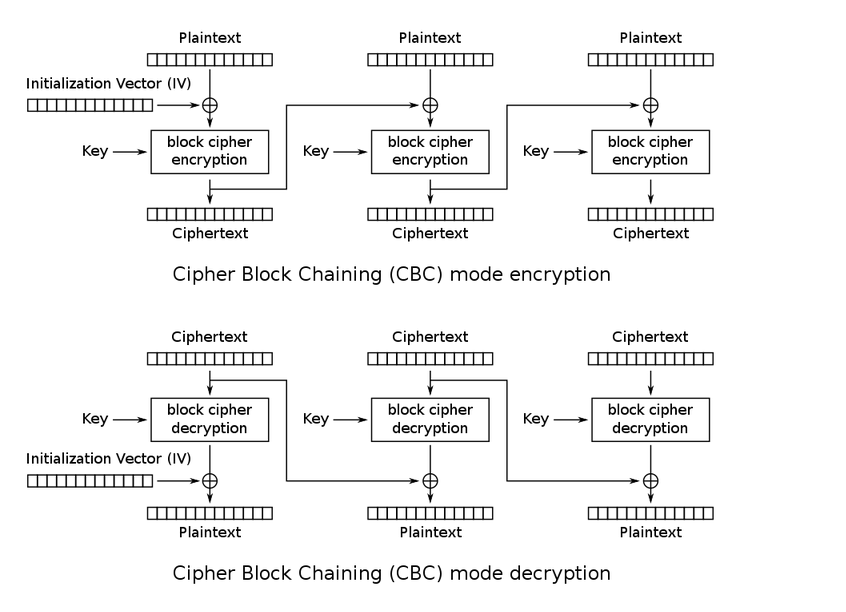
\includegraphics[scale=0.4]{imagenes/cbc.png} 
			\caption{Esquema del cifrado y descifrado del modo CBC \cite{cifradobloque}.}
			\label{esquemahtb}
		\end{figure}

	\item \textbf{Cipher FeedBack}
	\begin{itemize}
		\item \textbf{\emph{Cifrado CFB}}
		\begin{description}
			\item $x_{[0]} \in \mathbb{B}^r$
			\item Dividimos m en $m_{[1]}...m_{[l]}$ con $m_{[i]} \in \mathbb{B}^N$
			\item Para i=1,...,l hacer
			\begin{description}
				\item $c_{[i]} = m_{[i]}\oplus msb_r(E_k(m_{[i]}))$
				\item $x_{[i+1]} = lsb_{N-r}(x_i)||c_{[i]$
			\end{description}
			\item Devolvemos $c_{[1]}...c_{[l]}$
		\end{description}

		\item \textbf{\emph{Descifrado CFB}}
		\begin{description}
			\item Dividimos c en $c_{[1]}...c_{[l]}$ con $c_{[i]} \in \mathbb{B}^r$
			\item Para i=1,...,l hacer
			\begin{description}
				\item $m_{[i]} = c_{[i]}\oplus msb_r(E_k(x_{[i]}))$
				\item $x_{[i+1]} = lsb_{N-r}(x_i)||c_{[i]$
			\end{description}
			\item Devolvemos $m_{[1]}...m_{[l]}$
		\end{description}
	\end{itemize}

%\newpage
		\begin{figure}[htb]
			\centering
			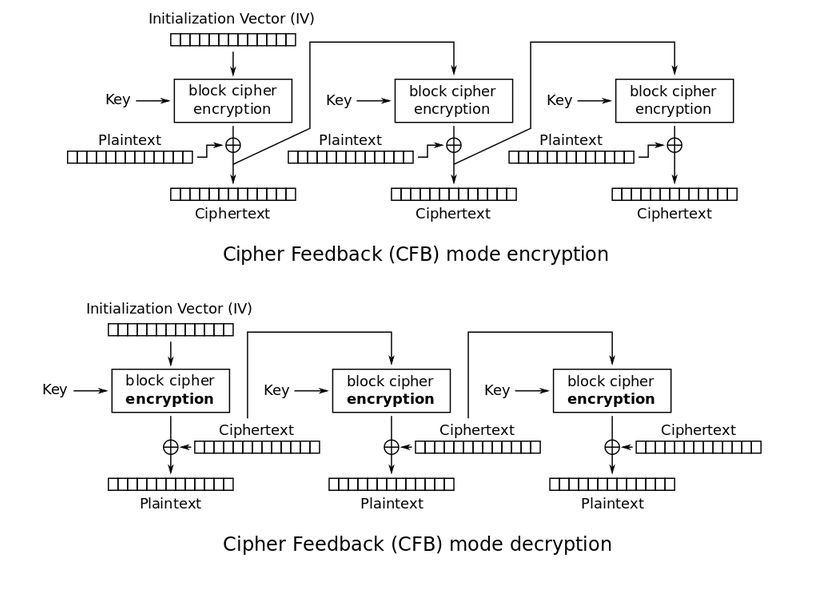
\includegraphics[scale=0.4]{imagenes/cfb.png} 
			\caption{Esquema del cifrado y descifrado del modo CFB \cite{cifradobloque}.}
			\label{esquemacfb}
		\end{figure}

	\item \textbf{Output FeedBack}
	\begin{itemize}
		\item \textbf{\emph{Cifrado OFB}}
		\begin{description}
			\item $x_{[0]} \in \mathbb{B}^N$
			\item Dividimos m en $m_{[1]}...m_{[l]}$ con $m_{[i]} \in \mathbb{B}^N$
			\item Para i=1,...,l hacer
			\begin{description}
				\item $x_{[i]} = E_k(x_{[i-1]})$
				\item $c_{[i]} = m_{[i]}\oplus x_{[i]}$
			\end{description}
			\item Devolvemos $c_{[1]}...c_{[l]}$
		\end{description}

%\newpage
		\item \textbf{\emph{Descifrado OFB}}
		\begin{description}
			\item Dividimos c en $c_{[1]}...c_{[l]}$ con $c_{[i]} \in \mathbb{B}^N$
			\item Para i=1,...,l hacer
			\begin{description}
				\item $x_{[i]} = E_k(x_{[i-1]})$
				\item $m_{[i]} = c_{[i]}\oplus x_{[i]}$
			\end{description}
			\item Devolvemos $m_{[1]}...m_{[l]}$
		\end{description}
	\end{itemize}
\end{itemize}

		\begin{figure}[htb]
			\centering
			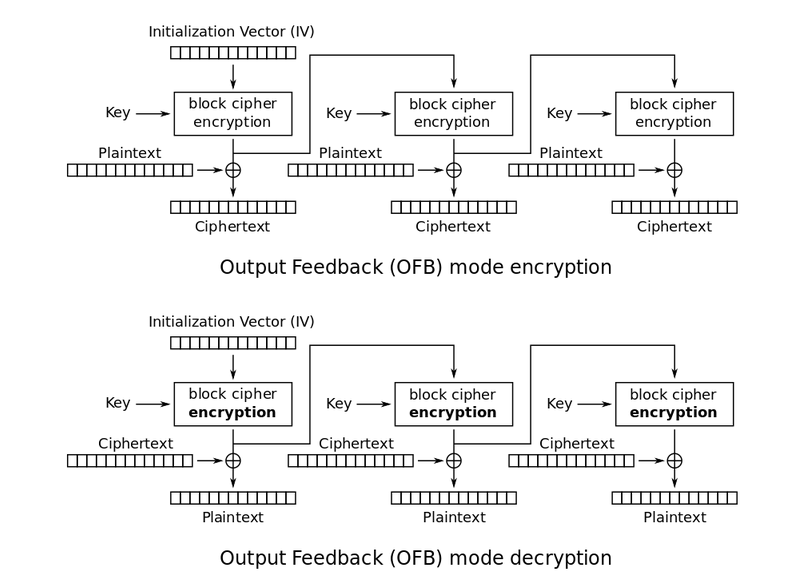
\includegraphics[scale=0.4]{imagenes/ofb.png} 
			\caption{Esquema del cifrado y descifrado del modo OFB \cite{cifradobloque}.}
			\label{esquemaofb}
		\end{figure}

\newpage
\section{El algoritmo Rijndael AES}
En esta sección hablaré sobre el cifrado Rijndael AES el cual es un cifrado de bloque simétrico muy utilizado actualmente por aplicaciones como \emph{Telegram}, \emph{WhatsApp} y \emph{FacebookChat} entre otras.\\
El algoritmo Rijndael llamado así en honor a sus dos autores Joan Daemen y Vicent Rijmen, es un algoritmo de cifrado por bloques que fue adoptado en octubre de 2000 por el NIST(\emph{National Institute for Standards and Technology}) para su empleo en aplicaciones criptográficas no militares en sustitución del algoritmo \emph{DES} después de un proceso de más tres años en los que se buscaba un algoritmo que fuera potente, eficiente y fácil de implementar.\\
Está diseñado para manejar longitudes de clave y de bloque variables entre los 128 y los 256 bits y aunque estos sean variables, en el estándar adoptado por el Gobierno de Estados Unidos en 2001 \cite{aesUsa} establece una longitud fija de bloque de 128 bits y una longitud de clave a escoger entre 128, 192 y 256 bits.\\
La información para los siguientes apartados de AES la he obtenido de \cite{GomezPardo2002b} para el primero y \cite{En2011} para el resto.\\
Como he mencionado anteriormente, AES es un cifrado de bloque, por lo que empezaré introduciendo que son los cifrados de bloque y los distintos modos de operación que tienen para así poder entender mejor el cifrado AES.


\subsection{Estructura de AES}
En el algoritmo AES se define cada ronda como una composición de cuatro funciones invertibles diferentes, formando tres \emph{capas}. Estas funciones tienen un propósito específico:
\begin{itemize}
	\item \textbf{Capa de mezcla lineal:} Formada por las funciones \emph{DesplazarFila} y \emph{MezclarColumnas} y permite obtener un alto nivel de difusión a lo largo de varias rondas.
	\item \textbf{Capa no lineal:} Formada por la función \emph{ByteSub} y es la aplicación paralela de s-cajas con propiedades óptimas de no linealidad.
	\item \textbf{Capa de adición de clave:} Es un simple \emph{or-exclusivo} entre el estado intermedio y la subclave correspondiente a cada ronda.
\end{itemize}

\subsection{Elementos de AES}
AES es un algoritmo que se basa en aplicar un número determinado de rodas a un valor intermedio denominado \emph{estado} que puede ser representado por una matriz rectangular que posee cuatro filas y $N_{b}$ columnas. Análogamente la clave tiene la misma estructura, una matriz de cuatro filas y $N_{k}$.
El bloque ha cifrar o descifrar se traslada directamente byte a byte sobre la matriz de estado de columna en columna($a_{0,0}, a_{1,0}, a_{2,0}, a_{3,0}, a_{0,1} ...$)

\begin{table}[htb]
	\begin{center}
		\begin{tabular}{| l | l | l | l |}
				\hline
				$\math{a}_{0,0}$ & $\math{a}_{0,1}$ & $\math{a}_{0,2}$ & $\math{a}_{0,3}$\\ \hline
				$\math{a}_{1,0}$ & $\math{a}_{1,1}$ & $\math{a}_{1,2}$ & $\math{a}_{1,3}$\\ \hline
				$\math{a}_{2,0}$ & $\math{a}_{2,1}$ & $\math{a}_{2,2}$ & $\math{a}_{2,3}$\\ \hline
				$\math{a}_{3,0}$ & $\math{a}_{3,1}$ & $\math{a}_{3,2}$ & $\math{a}_{3,3}$\\ \hline
		\end{tabular}
		\caption{Ejemplo de matriz de estado con $N_b=4$(128 bits).}
	\end{center}
\end{table}

\begin{table}[htb]
	\begin{center}
		\begin{tabular}{| l | l | l | l |}
				\hline
				$\math{k}_{0,0}$ & $\math{k}_{0,1}$ & $\math{k}_{0,2}$ & $\math{k}_{0,3}$\\ \hline
				$\math{k}_{1,0}$ & $\math{k}_{1,1}$ & $\math{k}_{1,2}$ & $\math{k}_{1,3}$\\ \hline
				$\math{k}_{2,0}$ & $\math{k}_{2,1}$ & $\math{k}_{2,2}$ & $\math{k}_{2,3}$\\ \hline
				$\math{k}_{3,0}$ & $\math{k}_{3,1}$ & $\math{k}_{3,2}$ & $\math{k}_{3,3}$\\ \hline
		\end{tabular}
		\caption{Ejemplo de clave con $N_k=4$(128 bits).}
	\end{center}
\end{table}

En otros casos el bloque y la clave pueden ser representados como vectores de registro de 32 bits donde cada registro esta compuesto por los bytes de la columna correspondiente ordenados en orden descendiente.\\

Siendo $B$ el bloque que queremos cifrar y $S$ la matriz de estado, el algoritmo AES con $n$ quedaría:

\begin{enumerate}
	\item Calcular $K_0, K_1,...,K_n$ subclaves a partar de la clave $K$.
	\item $S\leftarrow B \oplus K_0$
	\item Para $i=1$ hasta $n$ hacer
	\begin{description}
			\item Aplicar la roda \emph{i}-ésima del algoritmo con la subclave $K_i$
	\end{description}
\end{enumerate}
Como las funciones usadas en cada ronda son invertibles, para descifrar aplicaremos las funciones inversas de las funciones usadas para cifrar en el orden opuesto.

\begin{table}[htb]
	\begin{center}
		\begin{tabular}{| l | l | l | l |}
				\hline
				& $N_b = 4$(128 bits) & $N_b = 6$(192 bits)& $N_b = 8$(256 bits)\\ \hline
				$N_b = 4$(128 bits)& 10 & 12 & 14\\ \hline
				$N_b = 6$(128 bits)& 12 & 12 & 14\\ \hline
				$N_b = 8$(128 bits)& 14 & 14 & 14\\ \hline
		\end{tabular}
		\caption{Número de rodas en función del tamaño de la clave y bloque}
		\label{rondas_aes}
	\end{center}
\end{table}

\subsection{Las Rondas de AES}
Dado que el algoritmo AES puede aplicarse para longitudes diferentes de bloque y clave, el número de rondas es variables, como se ha visto en \ref{rondas_aes}.\\
Siendo $S$ la matriz de estado y $K_i$ la subclave correspondiente a la ronda $i$-ésima, cada ronda posee esta estructura:
\begin{enumerate}
	\item $S \leftarrow ByteSub(S)$
	\item $S \leftarrow DesplazarFila(S)$
	\item $S \leftarrow MezclarColumnas(S)$
	\item $S \leftarrow K_i \oplus S$
\end{enumerate}
En la última ronda se hacen solo los tres primeros pasos del algoritmo.

\begin{description}
	\item \textbf{ByteSub}\\
		La función \emph{ByteSub} es una sustitución no lineal que se aplica a cada byte de la matriz de estado mediante una s-caja 8\texttimes8. Se obtiene componiendo dos transformaciones:
		\begin{enumerate}
			\item Cada byte se considera como un elemento del $GF(2^8)$ generado por el polinomio irreducible $m(x)=x^8+x^4+x^3+x+1$ y es sustituido por su inversa multiplicativa quedando el valor cero inalterado. 
			\item A continuación se aplica la siguiente transformación afín en $GF(2)$ siendo $x_0, x_1,...,x_7$ los bits del byte correspondiente e $y_0, y_1,...,y_7$ los del resultado:

				\begin{equation*} 
					\begin{bmatrix} 
						y_0\\
						y_1\\
						y_2\\
						y_3\\
						y_4\\
						y_5\\
						y_6\\
						y_7\\
					\end{bmatrix}
					=
					\begin{bmatrix} % O matrices como esta de 4 x 3
						1 & 0 & 0 & 0 & 1 & 1 & 1 & 1\\
						1 & 1 & 0 & 0 & 0 & 1 & 1 & 1\\
						1 & 1 & 1 & 0 & 0 & 0 & 1 & 1\\
						1 & 1 & 1 & 1 & 0 & 0 & 0 & 1\\
						1 & 1 & 1 & 1 & 1 & 0 & 0 & 0\\
						0 & 1 & 1 & 1 & 1 & 1 & 0 & 0\\
						0 & 0 & 1 & 1 & 1 & 1 & 1 & 0\\
						0 & 0 & 0 & 1 & 1 & 1 & 1 & 1\\
					\end{bmatrix}
					\begin{bmatrix}
						x_0\\
						x_1\\
						x_2\\
						x_3\\
						x_4\\
						x_5\\
						x_6\\
						x_7\\
					\end{bmatrix}
					+
					\begin{bmatrix}
						1\\
						1\\
						0\\
						0\\
						0\\
						1\\
						1\\
						0\\
					\end{bmatrix}
			\end{equation*}
		\end{enumerate}
		La función inversa de $ByteSub$ es la aplicación inversa de la s-caja de cada byte de la matriz de estado.

	\item \textbf{DesplazarFila}\\
		Esta función desplaza a la izquierda de manera cíclica las filas de la matriz de estado. Cada fila $f_i$ se desplaza un número de posiciones $c_i$ diferente. Mientras que $c_0$ siempre es igual a cero, el resto de valores vine en función de $N_b$ como se puede ver en \ref{ciennb}.\\
		La función inversa será el desplazamiento de las filas de la matriz el mismo número de posiciones pero en el sentido contrario.

		\begin{table}[htb]
			\begin{center}
				\begin{tabular}{| l | l | l | l |}
						\hline
						$N_b$ & $c_1$ & $c_2$ & $c_3$\\ \hline
						4 & 1 & 2 & 3\\ \hline 
						6 & 1 & 2 & 3\\ \hline 
						8 & 1 & 3 & 4\\ \hline 
				\end{tabular}
				\caption{Valores de $c_i$ según el tamaño de bloque $N_b$}
				\label{ciennb}
			\end{center}
		\end{table}

		\begin{figure}[htb]
			\centering
			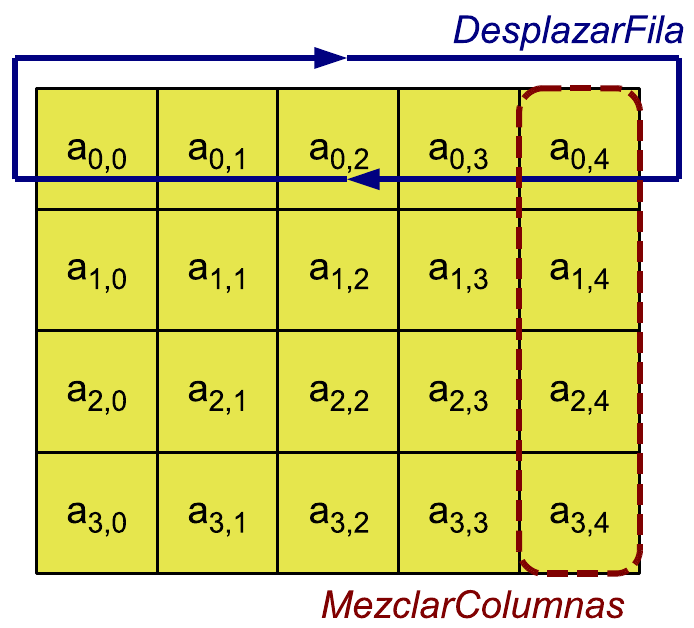
\includegraphics[scale=0.4]{imagenes/aesdesplazarmezclar.png} 
			\caption{Esquema de las funciones $MezclarColumnas$ y $DesplazarFila$ \cite{En2011}}
			\label{desplazarymezclar}
		\end{figure}
\newpage
	\item \textbf{MezclarColumnas}\\
		Durante la aplicación de esta función se considera cada columna del vector de estado se considera un polinomio cuyos coeficientes pertenecen a $GF(2^8)$ y se multiplica módulo $x^4+1$ por: $c(x)=03x^3+01x^2+01x+02$ donde 03 es el valor hexadecimal que se obtiene concatenado los coeficientes binarios del polinomio correspondiente en $GF(2^8)$, en este caso sería 00000011 y por tanto $x+1$ análogamente se haría con los demás.\\
		La inversa de $MezclarColumnas$ se obtiene multiplicando cada columna de la matriz de estado por el polinomio: $d(x)=0Bx^3+0Dx^2+09x+0E$

\end{description}

\subsection{Cálculo de las Subclaves}
Las subclaves $K_i$ se obtienen de la clave principal $K$ mediante el uso de dos funciones: una de expansión y otra de selección. Siendo $n$ el número de rondas que se van a aplicar, la función de expansión obtiene a partir del valor de $K$ una secuencia de $4(n+1)N_b$ bytes.\\
La función de selección toma consecutivamente de la secuencia obtenida bloques del mismo tamaño que la matriz de estado y los asigna a cada $K_i$.\\

Sea $K(i)$ un vector de bytes de tamaño $4N_k$ conteniendo la clave y sea $W(i)$ un vector de $N_b(n+1)$ registros de 4 bytes, siendo $n$ el número de rondas. 
La función de expansión tiene dos versiones según el valor de $N_k$:

\begin{itemize}
	\item Si $N_k<=6$:
	\begin{algorithm}
		Para $i$ desde 0 hasta $N_{k}-1$ hacer:
		\begin{description}
			$W(i)\leftarrow(K(4·i), K(4·i+1), K(4·i+2), K(4·i+3))$
		\end{description}
		Para $i$ desde $N_k$ hasta $N_{b}·(n+1)$ hacer:\\
			\hspace*{20}$tmp\leftarrow W(i-1)$\\
			\hspace*{20}Si $i$ $mod N_k == 0$\\
			\hspace*{40}$tmp\leftarrow Sub(Rot(tmp))\oplus Rc(i/N_k)$\\
			\hspace*{20}$W(i)\leftarrow W(i-N_k)\oplus tmp$
	\end{algorithm}

	\item Si $N_k>6$:
	\begin{algorithm}
		Para $i$ desde 0 hasta $N_{k}-1$ hacer:
		\begin{description}
			$W(i)\leftarrow(K(4·i), K(4·i+1), K(4·i+2), K(4·i+3))$
		\end{description}
		Para $i$ desde $N_k$ hasta $N_{b}·(n+1)$ hacer:\\
			\hspace*{20}$tmp\leftarrow W(i-1)$\\
			\hspace*{20}Si $i$ $mod N_k == 0$\\
			\hspace*{40}$tmp\leftarrow Sub(Rot(tmp))\oplus Rc(i/N_k)$\\
			\hspace*{20}Si $i$ $mod N_k == 4$\\
			\hspace*{40}$tmp\leftarrow Sub(tmp)$\\
			\hspace*{20}$W(i)\leftarrow W(i-N_k)\oplus tmp$
	\end{algorithm}
\end{itemize}

La función \emph{Sub} devuelve el resultado de aplicar la s-caja de AES a cada uno de los bytes del registro de cuatro que se le pasa como parámetro, la función \emph{Rot} desplaza a la izquierda los bytes del registro y \emph{Rc(j)} es una constante que se define como:
\begin{itemize}
	\item $Rc(j)=(R(j),0,0,0)$
	\item Cada $R(i)$ es el elemento de $GF(2^8)$ correspondiente al valor $x^{i-1}$ módulo $x^8+x^4+x^3+x+1$
\end{itemize}

\section{Criptosistema de Rivest-Shamir-Adleman, RSA}
En esta sección hablaré sobre el cifrado RSA y su funcionamiento, cifrado que como AES, está muy extendido y es utilizado por muchas aplicaciones para cifrar y validar los mensajes.\\
RSA es llamado así en honor a sus creadores Ron Rivest, Adi Shamir y Loenard Adleman, fué desarrollado en 1977. Cabe a destacar que en 1973 se desarrolló en secreto un criptosistema similar por Clifford Cocks para la \emph{Government Communications Headquarters}, que es la agencia de inteligencia de señales británica, y fue desclasificado en 1997\cite{cliffordCocks}.\\
Este criptosistema está basado en el \emph{Teorema de Euler} y en particular en la \emph{proposición 2.2}.
\begin{teorema}
	(Teorema de Euler) Sean a,n $\in \mathbb{Z}$ primos relativos entre sí, entonces $a^{\phi(n)}\equiv 1$ mod n.
\end{teorema}
Donde $\phi(n)$ es la \emph{funclón de Euler} definida como $\phi(n)=|\mathbb{Z}^*_n|$ y se puede calcular de la siguiente forma $$\phi(n)=n\prod_{p_i|n}(1-\frac{1}{p_i})$$


\begin{proposicion}
	Sea $n = pq$, donde p y q son dos primos distintos. Si $x\equiv 1$ mod $\phi(n)$, entonces $a^x\equiv a$ mod n $\forall a \n \in \mathbb{Z}$.\\
	\begin{proof}
		\textbf{Demostración.}\\
		Si a es múltiplo de n, entonces se cumple que $a^x \equiv 0 \equiv a$ mod n. Si a y n son coprimos, $mcm(a,n) = 1$ entonces tendríamos que $a^x \equiv a$ mod n por el Teorema de Euler.\\
		Nos quedaría ver ocurre en el caso de a sea múltiplo de p o de q, pero no de ambos. Por simetría supondremos que a es múltiplo de p, pero no de q. En este caso tenemos que $a^x \equiv 0 \equiv a$ mod p  y $a^x \equiv a$ mod q por el Teorema de Fermat, como p y q son coprimos entre sí, aplicando el Teorema Chino de los Restos se deduce que $a^x \equiv a$ mod n. \blacksquare
	\end{proof}
\end{proposicion}

\subsection{Descripción de RSA}
El funcionamiento de RSA lo he obtenido de \cite{angelRiosMateos} y es el siguiente:\\
El usuario elige dos números primos distintos \emph{p} y \emph{q} de buen tamaño ya que mientras más grandes sean más seguro será el cifrado.
Se calcula $n = pq$ y $\phi(n) = (p-1)(q-1)$, a continuación se elige un elemento $c \in \mathbb{Z}_{\phi(n)}^*$ y se calcula el inverso \emph{d}, de \emph{c} en $\mathbb{Z}_{\phi(n)}$. La clave pública será $k=(n,c)$ y la clave privada $k'=(n,d)$.\\
En un principio se consideraba que un tamaño de $n$ de 1024 bits era lo suficientemente grande para que fuera seguro, pero en 2003 Tromer y Shamir mostraron que es posible factorizar números de 1024 bits \cite{1024RSA} por lo que en la actualidad se considera 2048 bits como un tamaño seguro.\\
El conjunto de los mensajes sin cifrar es $\mathcal{M}$, el de los mensajes cifrados será $\mathcal{C}$ y se verifica que $\mathcal{M} = \mathcal{C} = \mathbb{Z}_n$ y las funciones de cifrado y descifrado serán respectivamente:
\begin{align*}
	E_{k}:\mathcal{M}\rightarrow\mathcal{C}\\
	a \rightarrow a^c
\end{align*}
\begin{align*}
	D_{k'}:\mathcal{C}\rightarrow\mathcal{M}\\
	a \rightarrow a^d
\end{align*}

\subsection{Ataques}
Como hemos visto anteriormente RSA puede ser vulnerable en función de los números primos que se elijan y el tamaño de estos. En este apartado veremos algunos posibles ataques que se podrían llevar a cabo \cite{GomezPardo2002b}.
\begin{description}
	\item \textbf{Ataque por módulo común.}\\
	Este ataque se da cuando hay una mala elección de las claves, típicamente cuando se tienen que generar múltiples claves para varios usuarios y para optimizar, se utiliza el mismo módulo $n$ para todos. Mientras el exponente sea distinto, la clave sigue siendo segura, pero si se da que se cifra el mismo mensaje con los distintos exponentes pero el mismo módulo, se puede descifrar el mensaje original.\\
	Supongamos que tenemos dos claves públicas con el mismo módulo, $(n, e_1)$ y $(n, e_2)$ y además ser verifica que  $mcm(e_1,e_2)$. Supongamos que $re_1+se_2=1$ con $r$\textless $0$\textless $s$. Como se ha visto el mensaje cifrado respectivamente será:
	\begin{align*}
		c_1 = m^{e_1} \mod n\\
		c_2 = m^{e_2} \mod n
	\end{align*}
	Si $(c_1,n) \neq 1$, podemos factorizar $n$ y romper la clave, por lo que podemos suponer que $c_1 \in \mathcal{U}(\mathbb{Z}_n)$. Calculamos $c_1^{-1}$ con el algoritmo extendido de Euclídes tenemos que :
	\begin{align*}
			(c^{-1})^{-r}c_2^s \equiv (m^{e_1})^r(m^{e_2})^s \equiv m^{e_1r+e_2s} = m \mod n
	\end{align*}

	\item \textbf{Ataque por exponente pequeño.}\\
	Este ataque se puede hacer cuando se elige un exponente muy pequeño y se cifra el mismo mensaje con distinto módulo. En este caso se puede resolver aplicando el Teorema Chino del Resto. Supongamos a varios receptores con claves públicas $(n_i, e)$, con $1\leq i \leq r$, tal que mcm$(n_i, n_j) = 1$ si $i\neq j$ ya que en caso contrario, se podría factorizar el módulo correspondiente mediante el cálculo del MCD.\\
	Llamamos $c_i = m^e \mod n_i$ para cada $1\leq i \leq r$. Seleccionamos $\{i_1,...,i_e \}\subseteq \{1,...,r\}$ y empleando el inverso del isomorfismo de anillos
	\begin{align*}
		\chi:\mathbb{Z}_{n_{i_1}...n_{i_e}}\rightarrow \mathbb{Z}_{n_{i_1}}\times ... \times \mathbb{Z}_{n_{i_e}}
	\end{align*}
	obtenido gracias al Teorema Chino del Resto, se puede calcular
	\begin{align*}
		\chi^{-1}(c_{i_1},...,c_{i_e}) = m^e \mod n_{i_1},....n_{i_e}
	\end{align*}
	Dado $m^e$\textless $n_{i_1}...n_{i_e}$, se puede obtener $m$ calculando la raíz $e$-ésima en $\mathbb{Z} \subseteq \mathbb{R}$, siempre y cuando $e$ no sea muy grande.

	\item \textbf{Ataque con primos muy próximos.}\\
	Este ataque se da cuando se eligen dos primos muy próximos entre sí. Dado $n=pq$ con $p$\textless $q$ tenemos que  
	\begin{align*}
			n=\left (\frac{p+q}{2}\right )^2-\left (\frac{p-q}{2}\right )^2
	\end{align*}
	Si $p$ y $q$ son cercanos, $s=\frac{p-q}{2}$ es pequeño y $t=\frac{p+q}{2}$ es un entero ligeramente mayor que $\sqrt{n}$ tal que $t^2 - n^2$ es un cuadrado perfecto. Probando sucesivamente con valores mayores que $\sqrt{n}$ hasta encontrar una descomposición $n=t^2-s^2$, tenemos que $p=t+s$ y $q=t-s$.
\end{description}

\subsection{Firma digital RSA}
Una vez explicado RSA se introducirá la firma digital con RSA, herramienta muy utilizada en las aplicaciones de mensajería para garantizar el no repudio de los mensajes.
Dados dos interlocutores A y B cada uno con sus claves públicas:
\begin{itemize}
	\item Para A tenemos $n_A$, $d_A$ y $e_A$   
	\item Para B tenemos $n_B$, $d_B$ y $e_B$   
\end{itemize}
Para que B sepa que un mensaje \emph{m} ha sido enviado por A se siguen los siguientes pasos:
\begin{enumerate}
	\item A cifra el mensaje \emph{m} usando su clave secreta.
		$$
			S=D_A(m)=m^{d_A} \mod n_A
		$$
	\item A continuación encripta el mensaje firmado con la clave pública de B.
		$$
			C_B(S)=S\mod n_B
		$$
		Y se lo envía.
	\item B recibe $C_B(S)=S^{e_B}$ y lo desencripta. 
		$$
			D_B(S^{e_B})=S \mod n_B
		$$
	\item Una vez desencriptado la primera parte, B desencripta S con la clave pública de A.
		$$
			C_A(S)=C_A(D_A(m))=(m^{d_A})^{e_A}=m^{d_Ae_B}=m^{1+k\phi(n_A)}\equiv m \mod n_A
		$$
\end{enumerate}
Una vez hecho esto, B podría afirmar casi con total seguridad que el mensaje ha sido enviado por A garantizando el no repudio del mensaje.

\section{Criptosistemas basados en el logaritmo discreto. Diffie-Hellman}
Una vez visto RSA veremos a continuación una introducción a los criptosistemas basados en el problema del logaritmo discreto que nos permitirá definir el intercambio de claves \emph{Diffie-Hellman}, método muy utilizado en las aplicaciones de mensajería al inicio de las conexión. La información de este apartado sobre el logaritmo ha sido obtenida de \cite{angelRiosMateos} y la de \emph{Diffie-Hellman} ha sido obtenida de \cite{En2011}.\\
El problema del logaritmo discreto es definido de la siguiente forma:
\begin{definicion}
	Sea S un semigrupo finito. El Problema del Logaritmo Discreto en el semigrupo S es el de resolver ecuaciones del tipo\\
		$$
			a^X\!=b\;(x\in \mathbb{N})
		$$
	donde a y b son dos elementos dados de S.
\end{definicion}

La complejidad del problema del Logaritmo discreto depende en gran medida del semigrupo $S$ que se elija.
Dado que si se eligiera como $S$ el grupo aditivo $\mathbb{Z}_n$ la solución se obtendría fácilmente resolviendo una ecuación de congruencias del tipo $aX \equiv b \mod n$ que equivaldría a resolver la ecuación diofántica $aX + nY = b$. Pero si ahora $S$ pasara a ser los semigrupos multiplicativos $\mathbb{Z}_n$ o $\mathbb{F}_q$ o sus grupos de unidades, el problema aumentaría su complejidad de manera significativa.\\
Tenemos que $a^x = b$ tiene solución si y solamente si $b$ está en el semigrupo cíclico generado por $a$. Luego si $a$ es un elemento de orden finito de un grupo, se podría suponer en la práctica que $S$ es un grupo cíclico y por ello existiría un isomorfismo con ($\mathbb{Z}_n$, $+$). Luego la dificultad del problema no estaría en la estructura del grupo, sino en reconocer los elementos como potencias de enteros.\\
Se cree que el problema de logaritmo discreto es $\mathbb{NP}$-completo, pero esta conjetura todavía no ha sido demostrada por lo que se considera un problema $\mathbb{NP}$-Intermedio, estos problemas son llamados así porque no están dentro de los problemas $\mathbb{P}$ ni en los problemas $\mathbb{NP}$-completo por ahora \cite{NP-intermedio}.\\
Una vez visto el problema de logaritmo discreto, se explicará el intercambio de claves \emph{Diffie-Hellman}.
\subsection{Intercambio de claves Diffie-Hellman}
Antes de explicar el intercambio de claves \emph{Diffie-Hellman} se introducirá el problema de Diffie-Hellman ya que es la base de este.\\

\begin{definicion}
	Dado el conjunto $\mathbb{Z}^*_{p'}$ con p primo, diremos que $\alpha \in \mathbb{Z}^*_p$ es un generador de $\mathbb{Z}^*_{p'}$ si se cumple:\\
	$$
		\forall b \in \mathbb{Z}^*_{p'},\: \exists i\: tal \: que \: \alpha^i = b
	$$
\end{definicion}

\begin{definicion}
	\textbf{(El Problema Diffie-Hellman)} Dado un número primo p, un número $\alpha$ que sea un \emph{generador} de $\mathbb{Z}^*_{p'}$, $\alpha^a$ y $\alpha^b$, encontrar $\alpha^{ab} \mod p$.  
\end{definicion}

\textbf{Intercambio de claves \emph{Diffie-Hellman}}\\
El intercambio de claves \emph{Diffie-Hellman} es un algoritmo asimétrico basado en el problema de \emph{Diffie-Hellman}, empleado para acordar una clave común en un canal inseguro. Los pasos que se siguen son:\\
Sean $A$ y $B$ dos interlocutores que quieren compartir un valor $K$. Para ello se calcula un número primo $p$ y un generador \alpha de $\mathbb{Z}^*_{p'}$ con $2\leq \alpha \leq p-2$. Esta información es pública y conocida por ambos.
\begin{enumerate}
	\item $A$ escoge un número aleatorio $x$, comprendido entre 1 y $p-2$ y envía a $B$ el valor 
		$$
			\alpha^x \mod p
		$$
	\item Análogamente $B$ escoge un número aleatorio $y$, comprendido entre 1 y $p-2$ y envía a $A$ el valor 
		$$
			\alpha^y \mod p
		$$

	\item $B$ recoge $\alpha^x$ y calcula $K=(\alpha^x)^y \mod p$
	\item $A$ recoge $\alpha^y$ y calcula $K=(\alpha^y)^x \mod p$
\end{enumerate}
Puesto que $x$ e $y$ son conocidos solamente por $A$ y $B$ respectivamente, tenemos que al final solamente $A$ y $B$ acaban conociendo el valor de $K$.\\
A continuación se introducirá la teoría de curvas Elípticas ya que nos permitirá redefinir el intercambio de claves usando estas, generando un problema mucho más complejo y con mayor seguridad el cual es el que se utiliza en aplicaciones de mensajería como \textbf{WhatsApp} y \textbf{Telegram}.

\section{Curvas Elípticas en Criptografía}
La criptografía en curvas Elípticas es considerada como uno de los campos de las matemáticas con más futuro en la criptografía asimétrica.
Esto es debido a sus propiedades que dan lugar a problemas de una gran complejidad computacional análogos a los que presenta la aritmética modular. 
Esto permite que sean utilizadas en algunos algoritmos asimétricos como puede ser el intercambio de claves \emph{Diffie-Hellman} que se verá más adelante. A priori su 
estructura algebraica es más compleja que la de la aritmética modular sin embargo, al implementarlas suelen ser más eficientes y además, con claves más cortas alcanzan 
el mismo nivel de seguridad.\\
El uso de curvas elípticas en criptografía se presentó por primera vez en 1985 por Neal Koblitz y Víctor Miller de manera independiente.\\
La información para esta sección se ha obtenido de \cite{En2011}.

\subsection{Curvas Elípticas en $\mathbb{R}$}
\begin{definicion}
	Una curva definida en $\mathbb{R}$ es el conjunto de puntos del plano (x,y) que cumplen la siguiente ecuación:
$$
	y^2=x^3+ax+b
$$
Donde los coeficientes a,b $\in \mathbb{R}$ defininen de manera unívoca a la curva.
\end{definicion}
Algunas curvas en $\mathbb{R}$ son:

\begin{figure}[H]
	\centering
	\subfloat[\centering Curva $y^2=x^3-4x+1$]{{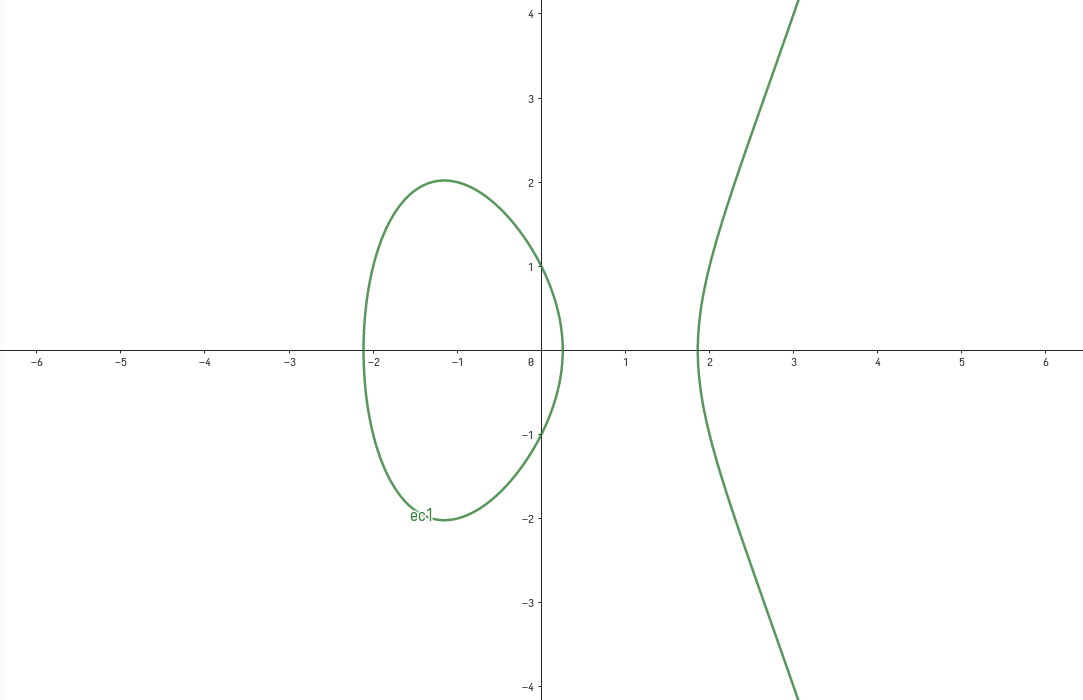
\includegraphics[width=5.9cm]{imagenes/ec1:y^2x^3-4x+1.png}}}
	\qquad
	\subfloat[\centering Curva $y^2=x^3-3x+4$]{{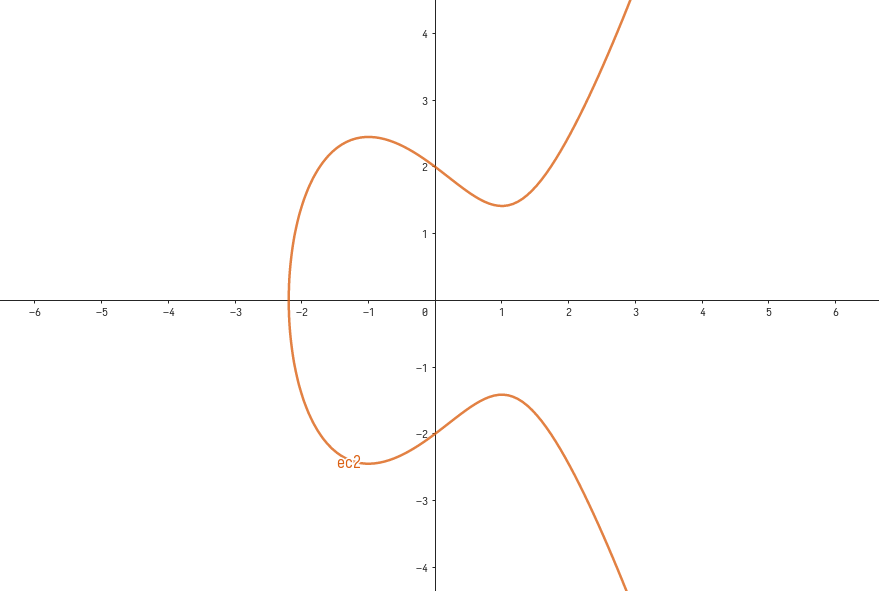
\includegraphics[width=5.9cm]{imagenes/ec2:y^2x^3-3x+4.png}}}
\end{figure}

Si se verifica que $x^3+ax+b$ no tiene raíces múltiples, tendremos que la curva junto con 
el punto $\mathcal{O}$ llamado \emph{punto en el infinito} y la operación $+$ que se definirá 
a continuación es lo que se denomina el \emph{grupo de curva elíptica E(\mathbb{R})}.\\
El punto $\mathcal{O}$ es un punto imaginario situado a una distancia infinita que no tendrá ningún valor en particular.\\

\textbf{Operación $+$ en $\mathbb{R}$}\\
Definido el conjunto en el que se trabajará, definiremos una ley de composición interna $+$.\\
Sean los puntos $r=(r_x,r_y)$, $s=(s_x,s_y)$, $p=(p_x,p_y)$, $t=(t_x,t_y)$ con $r,s,p,t \in E(\mathbb{R})$ la operación $+$ se define como sigue:
\begin{itemize}
	\item $r+\mathcal{O} = \mathcal{O}+r=r,\:\: \forall r \in E(\mathbb{R})$ .
	\item Si $r_x = s_x$ y $r_y = -s_y$, entonces $r=-s$ y además $r+s=s+r=\mathcal{O}$.
	\item Si $r\neq s$ y $r\neq -s$, $r+s=p$ donde $p$ será el opuesto del punto que corta la recta que une $r$ y $t$ con la curva.
	\item Para sumar un punto $p$ con sigo mismo si $p_y\neq0$ se usa la tangente de la curva en $p$. Luego tendremos que $t=p+p$ sera el opuesto de ese punto. Si $p_y=0$ entonces la tangente de la curva será perpendicular al eje de abcisas, por lo que se podría considerar que corta la curva en el infinito, luego $p+p=\mathcal{O}$.
	\item Para sumar $n$ veces un punto $p$ tenemos que si $p_y\neq 0$ entonces sumar $n$ veces $p$ será equivalente a multiplicar $p$ por el escalar $n$ y se representará como $np$. Si $p_y=0$ entonces la suma será:
\end{itemize}
\begin{aligned*}
	\center
	&$2r = r + r = \mathcal{O}$\\
	&$3r = 2r + r = \mathcal{O} + r = r$\\
	&$4r = 3r + r = r + r = \mathcal{O}$\\
	&...\\
\end{aligned}
La suma de curvas elípticas de manera algebraica se define de la siguiente forma:\\
Dados $r=(r_x,r_y)$ y $s=(s_x,s_y)$, tal que $r\noeq-s$, tenemos que $r+s=t$ donde $d=\frac{r_y-s_y}{r_x-s_x},\; t_x=d^2-r_x-s_x,\; t_y=-r_y+d(r_x-t_x)$.
De manera gráfica quedaría de la siguiente manera:\\
\begin{figure}[H]
	\centering
	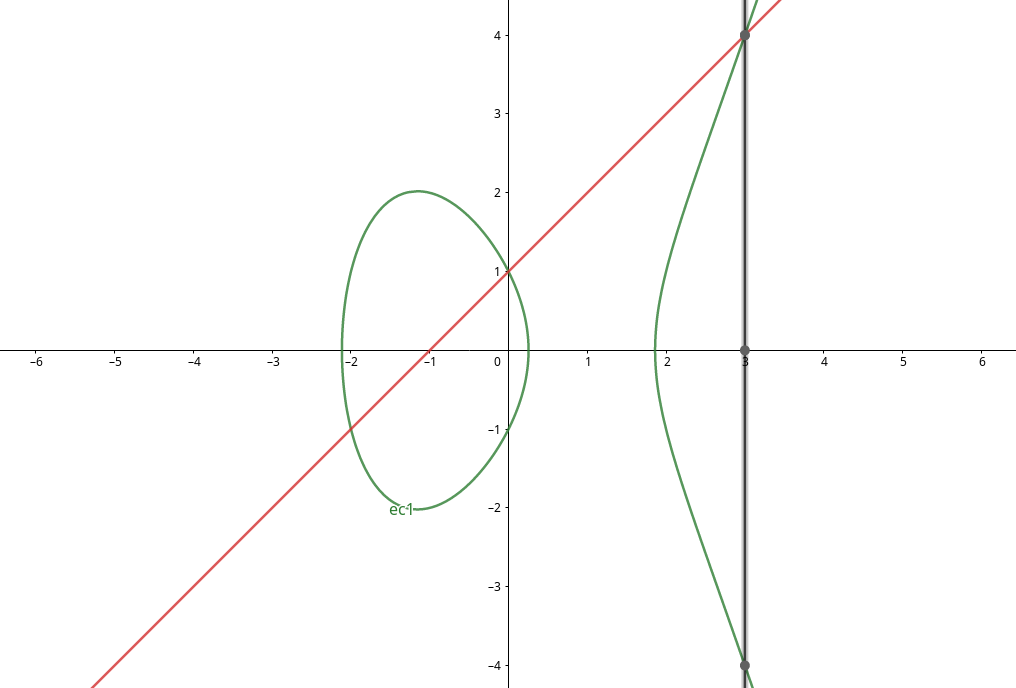
\includegraphics[scale=0.4]{imagenes/sumaCurva.png} 
	\caption{Suma en la curva $y^2=x^3-4x+1$ con $r=(-2,-1),\: s=(0,1),\: -t=(3,4)\: y \: t=(3,-4)$ }
	\label{esquemaecb}
\end{figure}

Una vez definidas las curvas elípticas en $\mathbb{R}$ definiremos las curvas en los cuerpos de Galois $GF(n)$ y $GF(2^n)$ cuyo uso esta muy extendido en la criptografía para redefinir el problema de logaritmo discreto.

\subsection{Curvas Elípticas en $GF(n)$}
Un cuerpo de Galois $GF(n)$ es el grupo finito generado por un número primo $n$. En este conjunto todos los elementos tienen un inverso, menos el cero por lo que están permitidas las operaciones de suma, resta, multiplicación y división.\\
De manera natural se define el conjunto $E(GF(n))$ como los puntos $(x,y)$ que verifican la siguiente ecuación: 
$$
	y^2\equiv x^3+ax+b \mod n
$$
Donde al igual que en $E(\mathbb{R})$, $a,b\in{1..n}$ definen de manera unívoca una curva elíptica.\\

\newpage
\textbf{Operación $+$ en $GF(n)$}\\
Sean los puntos $r=(r_x,r_y),\: s=(s_x,s_y),\: p=(p_x,p_y),\: t=(t_x,t_y)\in E(GF(n))$, definimos la operación $+$  como sigue:
\begin{itemize}
	\item $r+\mathcal{O}=\mathcal{O}+r=r,\: \forall r \in GF(n)$.
	\item Si $r_x=s_x$ y $r_y=s_x+s_y$, entoces se dice que $r$ es el opuesto de $s$, se nota como $r=-s$ y se verifica que $r+s=s+r=\mathcal{O}$.
	\item Si $r\neq s$ y $r\neq-s$, $t=r+s$ se calcula como $d=\frac{s_y-r_y}{s_x-r_x}\mod n,\; t_x=d^2-r_x-s_x \mod n,\; t_y=-r_y+d(r_x-t_x) \mod n$
	\item Si $p_x = 0$ entonces $2p = \mathcal{O}$
\end{itemize}

\subsection{El cuerpo de Galois $GF(2^n)$}

Antes de desarrollar las Curvas Elípticas en $GF(2^n)$ introduciré el cuerpo $GF(2^n)$ el cual tiene una serie de propiedades que lo hacen muy interesante y justifican su uso tan extendido en criptografía.\\
El conjunto $\mathbb{Z}_2[x]$ es el conjunto de polinomios con coeficientes en $\mathbb{Z}_2$ es decir, el el conjunto de polinomios cuyos coeficientes solo valen 0 o 1. Por lo que los polinomios pueden ser representados por una cadena de bits.
 Un ejemplo sería el polinomio $f(x)=x^4+x^3+x+1$ que quedaría representado como 11011. 
Además si lo sumamos con otro polinomio como puede ser $g(x)=x^2+x+1$ tenemos que $f(x)+g(x)=x^4+x^3+x^2$ que equivale a hacer la operación \emph{xor} entre 11011 y 00111, por lo que a nivel computacional, es muy fácil implementar estas operaciones.\\
Escogiendo un polinomio irreducible en $\mathbb{Z}_2$ podemos generar un cuerpo de Galois. Este conjunto es representado como $GF(2^n)$, donde $n$ es el grado del polinomio irreducible que lo genera.\\
Las principales ventajas que tiene trabajar con $GF(2^n)$ es que permite llevar a cabo implementaciones de una sencillez significativa respecto a la de los demás. Por lo que teniendo el mismo orden de complejidad, se multiplica significativamente la velocidad y además permite simplificar el diseño de los circuitos. Esto último hace que se obtengan sistemas con mejores prestaciones y mejor precio.

\subsection{Curvas Elípticas en $GF(2^n)$}

De manera análoga a $E(GF(n))$ definimos el conjunto $E(GF(2^n))$ con la diferencia debida a la estructura de $GF(2^n)$, la ecuación de curva elíptica es diferente.\\
Dado un polinomio irreducible $p(x)$ de grado $n$, las curvas elípticas se definen como los puntos $(x,y)$ que cumplen la ecuación:
$$
	y^2+xy \equiv x^3+ax^2+b \mod (p(x))
$$
y para que se genere un grupo se tiene que verificar que $b\neq 0$.
Los puntos de una curva serán pares de polinomios de grado $n-1$ y como hemos visto en el apartado anterior, podrán ser representados como cadenas de bits.\\

\textbf{Operación $+$ en $E(GF(2^n))$}\\
Sean los puntos $r=(r_x,r_y),\: s=(s_x,s_y),\: p=(p_x,p_y),\: t=(t_x,t_y)\in E(GF(n))$, definimos la operación $+$  como sigue:
\begin{itemize}
	\item $r+\mathcal{O}=\mathcal{O}+r=r,\; \forall r \in E(GF(2^n))$
	\item Si $r_x=s_x$ y $r_y=s_x+s_y$, entoces se dice que $r$ es el opuesto de $s$, se nota como $r=-s$ y se verifica que $r+s=s+r=\mathcal{O}$.
	\item Si $r\neq s$ y $r\neq-s$, $t=r+s$ se calcula como $d=\frac{s_y-r_y}{s_x-r_x},\; t_x=d^2+d+r_x+s_x+a,\; t_y=d(r_x+t_x)+t_x+r_y$.
	\item Para $t=2p$ con $p_x\neq 0$ se calcula como $d=p_x+\frac{p_y}{p_x}, \: t_x=d^2+d+a, \: t_y=p_x^2+(d+1)t_x$.
	\item Si $p_x=0$ tenemos que $2p=\mathcal{O}$
\end{itemize}

\subsection{El problema del logaritmo discreto usando curvas elípticas}

\section{Diffie-Hellman usando Curvas Elípticas}

\section{Funciones Hash}
